\chapter{Biomechanics: fluid-structure interaction and cardiac Radiofrequency Ablation}
\label{cha_rfa}
The rest of this thesis is devoted to biomechanics and a specific
application to which I devoted a good share, if not the lion's share,
of my time during my PhD: cardiac simulation with radiofrequency
ablation.

\section{Predictive Real Unified Continuum Simulation of biomechanics}

Here I give an overview of the predictive Real Unified Continuum (RUC)
cG(1)cG(1) Direct FEM Simulation methodology [ref], allowing general
phenomena such as multiphase fluid-structure interaction (FSI),
general interface motion, implicit contact, fracture, plasticity,
etc., The methodology also allows application of Direct duality-based
adaptive error control, which we will investigate in future work. RUC
is a generalization of the Unified Continuum framework which we
developed previously in [ref].

This work is developed as part of the Digital Math framework [ref] - as
the foundation of modern science based on constructive digital
mathematical computation.

The formulation allows mesh motion, similar to an
Arbitrary-Lagrange-Eulerian (ALE) setting, and mesh modification, and
importantly allows part or the entire mesh to be fixed, representing
zero mesh velocity. The demonstration cases below have been computed
with zero mesh velocity to investigate the limits of this setting.

\subsection{Real Unified Continuum Simulation}

The methodology is a Direct FEM simulation of the first principle
equations, here in multi-phase incompressible form, where we include
constitutive laws for a Newtonian fluid and Neo-Hookean solid.

These first principle equations are discretized by the Direct FEM
approach, meaning Galerkin-Least-Squares (GLS) stabilization with
shock-capturing.

The Galerkin part of the method is formulated as below in FEniCS
notation:

\begin{lstlisting}
F_G = z*inner(u, grad(rho))*nu*dx
F_G += z*(inner(rho*grad(u)*u + grad(p),v) - \
  theta*inner(sigma, grad(v)) + nnu*inner(grad(u),grad(v)) - \
  rho*dot(f,v))*dx
F_G += z*(inner(dot(u, grad(sigma)) + \
  theta*(2*rho*mumu*epsilon(u) + grad(u)*sigma + sigma*grad(u).T), y))*dx
\end{lstlisting}

and in corresponding strong form in Latex notation:	  
\begin{equation*} %\label{eq:nseinc2}
      \begin{array}{rcll} 
	    \rho (\partial_t {\bf u} + ({\bf u} \cdot \nabla) {\bf u}) - \nabla \cdot \sigma &=& 0
      \,\, &\mbox{in } Q,\\ 
	    \nabla \cdot {\bf u} &=& 0  \,\, &\mbox{in }Q,\\
	    \partial_t \rho + ({\bf u} \cdot \nabla) \rho &=& 0  \,\, &\mbox{in }Q,\\
	    \partial_t \theta + ({\bf u} \cdot \nabla) \theta &=& 0  \,\, &\mbox{in }Q,\\
            \sigma &\equiv& \bar{\sigma} - pI\\
            \bar{\sigma}_f &\equiv& 2\mu_f \epsilon\\
            \bar{\sigma} &\equiv& \theta \bar{\sigma}_f + (1 - \theta) \bar{\sigma}_s\\
            \partial_t \bar{\sigma}_s - 2\mu_s \epsilon - \nabla {\bf u} \bar{\sigma}_s - \bar{\sigma}_s \nabla {\bf u}^{\top} &=& 0
      \end{array} 
\end{equation*}   

\subsection{Application: Human heart}

With RUC We investigate a fully FSI canonical heart model, with
elastic heart walls and valves, driven by a force compressing the
heart walls. We observe a pumping motion with opening and closing of
the valves, and implicit contact in the valves.

\begin{wrapfloat}{figure}{O}{0pt}
  \centering
    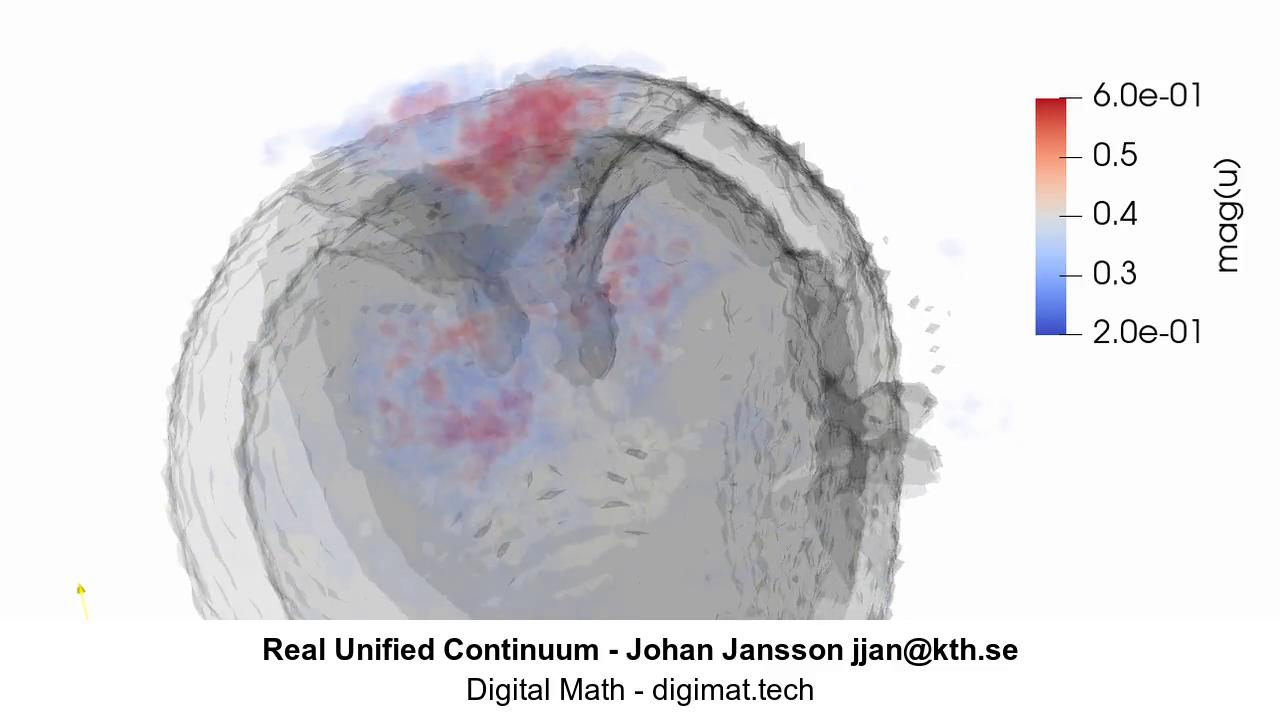
\includegraphics[width=0.5\columnwidth]{img/RealUnifiedContinuum-h107-heart-transparent-valves01.jpg}
    \caption{Real Unified Continuum Simulation of a canonical heart with valves.}
    \label{fig_rfa_catheter}
\end{wrapfloat}


\section{Radiofrequency ablation}
\label{sec_rfa}
Radiofrequency ablation is a minimally invasive treatment in which a catheter is used to deliver heat to a target tissue with the goal of burning it.
Heat is delivered by an electric current at a radio frequency of about \SI{500}{\kHz}, whence the name of the procedure, and is used to permanently damage the tissue of the patient in a very localised manner.
However counterproductive this might seem, it is not, and radiofrequency ablation is routinely used to treat a number of conditions such as hyperopia, asthma, gastric reflux, hepatic tumor, apnoea and, last but not least, cardiac arrhythmia.
The general idea of radiofrequency ablation is that causing controlled lesions in a tissue can be used to cure worse conditions, making it the lesser of two evils; some cardiac arrhythmias, for example, are caused by electric impulses propagating in the heart to areas where they should not, eliciting muscular contractions that affect the correct pace of the heart.
Burnt tissue, however, is known to be electrically insulating.
We can thus affect the electric circuit in a patient's heart, and in particular we can cut unwanted branches, by generating lesions that form a barrier that electricity cannot cross.

Not all treatments are equally safe, and the treatment of cardiac disorders is by far the most prone to risks and complications, even life-threatening: on average, around \SI{5}{\percent} of the administrations of cardiac radiofrequency ablation result in unexpected complications, a much higher rate than the other use cases mentioned above.

The risks with cardiac radiofrequency ablation, from now on \emph{RFA}, include the formation of cloths (or thrombi), when heat coagulates blood, and steam pop formation, arising when the temperature of the tissue is high enough that the water inside it evaporates.
Both scenarios are bad: thrombi have the potential to obstruct blood vessels if they accumulate in the circulatory system, but steam pops result in perforations of the cardiac wall.
When the perforation is transmural, meaning it pierces the heart from side to side, the patient's life is in great danger.
The pop is so violent it can literally be heard from outside the patient's body by the doctors in the room.
As a guideline, we consider that thrombi form in the blood when it reaches \SI{80}{\celsius}, while steam pop occur in the tissue at a temperature of \SI{100}{\celsius}; in contrast, tissue is considered irreversibly damaged at a temperature of \SI{50}{\celsius}.
The goal is then to bring a large enough portion of cardiac tissue to a temperature of \SI{50}{\celsius} while keeping the blood temperature below \SI{80}{\celsius} and the tissue temperature below \SI{100}{\celsius}.

RFA is administered to a patient that, although sedated, is still awake, and the doctor performing the procedure pushes the catheter through the patient's body, entering from the hip, manually applying pressure.
Several factors account for a less than ideal situation, most importantly the facts that the patient is not completely still -- his heart is beating -- and the doctor's pressure is not constant in time.
All these contribute to the high variability in the quality of the results of the procedure: although several different protocols are common, sometimes the lesions are too small, not blocking electricity properly and requiring a second administration, while sometimes too much power is delivered, resulting in complications.
On top of it, during the administration of the procedure it is hard to assess what is going on inside the patient, as inspecting the size of the lesion that is forming in the tissue is all but easy.
It is clear that this scenario can benefit from the help of numerical simulations to better understand what happens at the patient during the procedure, and this is the mission we set off to accomplish.

\section{Lesion assessment}
\label{sec_rfaLesion}
RFA is administered according to protocols.
A \emph{protocol} is a combination of values for pressure, power and time such as (\SI{20}{g}, \SI{30}{W}, \SI{10}{s}) meaning that the catheter should be held with a pressure of 20 grams, delivering 30 Watts of energy for 10 seconds\footnote{The use of the word \emph{pressure} to refer to a quantity in grams is typical for this application.}.

Manufacturers of medical devices use models, to some extent, to advise medical doctors on what protocols to use for a session of radiofrequency ablation.
These models are quite coarse-grained, often combining all three parameters in a protocol with some regression technique used a posteriori on experimental data from tests on animal tissue.
Although they are better than nothing, these models suffer from the limitations caused by condensing too much information in a single number and lack physical connection to the real scenario.
A mathematical model that draws from physical principles has the potential to do better.

\section{Mathematical modelling}
\label{sec_rfaModel}
In this section I will go through the modelling intervention that we performed to build a so-called \emph{digital twin} of the RFA procedure.

\subsection{Governing equations}
\label{sub_rfaEquations}
The RFA process is a multi-physics system involving fluid flow, current flux and thermal diffusion.

We used the incompressible Navier-Stokes equations to describe the fluid flow, which we already encountered in Equation~\eqref{eq_ns} in Section~\ref{sec_cfd} but that I report for convenience:
\begin{equation}
  \left\{
    \begin{aligned}
      &\partial_{t} \vec{u} (\vec{u} \cdot \grad) \vec{u} - \div\sigma(\vec{u},p) = \vec{0} \\
      &\div \vec{u} = 0
    \end{aligned}
  \right.
  \label{eq_rfaNS}
\end{equation}
where \(\vec{u}\) is the velocity, \(p\) is the pressure and \(\sigma(\vec{u},p) = 2 \nu \sym\grad \vec{u}\) is the stress tensor.

The electrical potential can be described as the solution to a Poisson-type equation.
This is a good approximation because the characteristic time in the evolution of radiofrequency currents is much shorter than that of the other phenomena considered in this simulation, so we can assume that the electrical potential is quasi-static and avoid solving the whole Maxwell equations in favour of a simpler elliptic equation.
We have
\begin{equation}
  \div(\sigma(T)\grad\Phi) = 0
  \label{eq_rfaPotential}
\end{equation}
where \(\Phi\) is the electrostatic potential and \(\sigma(T)\) is the electrical conductivity, that we consider as a function of the temperature \(T\).\footnote{It is an unfortunate coincidence that both the stress tensor and the electrical conductivity are denoted by the letter \(\sigma\) in the literature of the respective fields, but in this work they have different arity so no confusion should arise.}
This equation has to be solved with an additional constraint: during the RFA procedure, the machine used to provide power to the catheter does so trying to keep the dissipated power to a constant value \(P\) -- the one that appears in the protocol.
Recalling that, in electrostatics, the dissipated power is given by \(P = \vec{E} \cdot \vec{J}\) where the electrostatic field is \(\vec{E} = -\grad\Phi\) and the electrostatic current is \(\vec{J} = \sigma \vec{E}\), Equation~\eqref{eq_rfaPotential} needs to be complemented with the constraint
\begin{equation}
  \int \sigma(T) \norm*{\grad\Phi}^2 = P
  \label{eq_rfaPowerConstraint}
\end{equation}

Finally, for heat dissipation we used a modification of Penne's bioheat equation that describes tissue heating by both convection and power dissipation from radiofrequency currents.
The final form, that we have been using in the model, reads
\begin{equation}
  \rho c(T) \left( \partial_{t} T + \vec{u} \cdot \grad T\right) - \div(k(T) \grad T) = \sigma(T) \norm*{\grad \Phi}^2
  \label{eq_rfaBioheat}
\end{equation}
featuring the density \(\rho\), the specific heat \(c\), the thermal conductivity \(k\) and the temperature \(T\).
\(\Phi\) and \(\sigma\) are the same as in Equation~\eqref{eq_rfaPotential} while \(\vec{u}\) is taken from Equation~\eqref{eq_rfaNS}.

\subsection{Catheter geometry}
\label{sub_rfaGeometry}
For this model we have been using a geometry based on the in vitro experiment that we want to reproduce.
The geometrical description, however, introduces a few improvements over the state of the art in these kinds of simulations.

First of all, the catheter geometry is quite complex in itself.
The outside of the catheter is an adiabatic body that insulates it thermally and electrically.
At its tip, however, there is an electrode on which the machine applies a potential difference to drive electric current.
Inside the electrode tip there is a glass piece, called \emph{thermistor}, that has a high thermal capacity and is used to keep the electrode's temperature low, preventing it from overheating.
Finally, at its core there is a channel that is used to inject coolant in the heart; to make things more complex, the channel has small outlets that pass through the thermistor and the electrode, in the count of six for the model used in the experiment.
We report an overview of the catheter geometry in Figure~\ref{fig_rfa_catheter}.
\begin{wrapfloat}{figure}{O}{0pt}
  \centering
    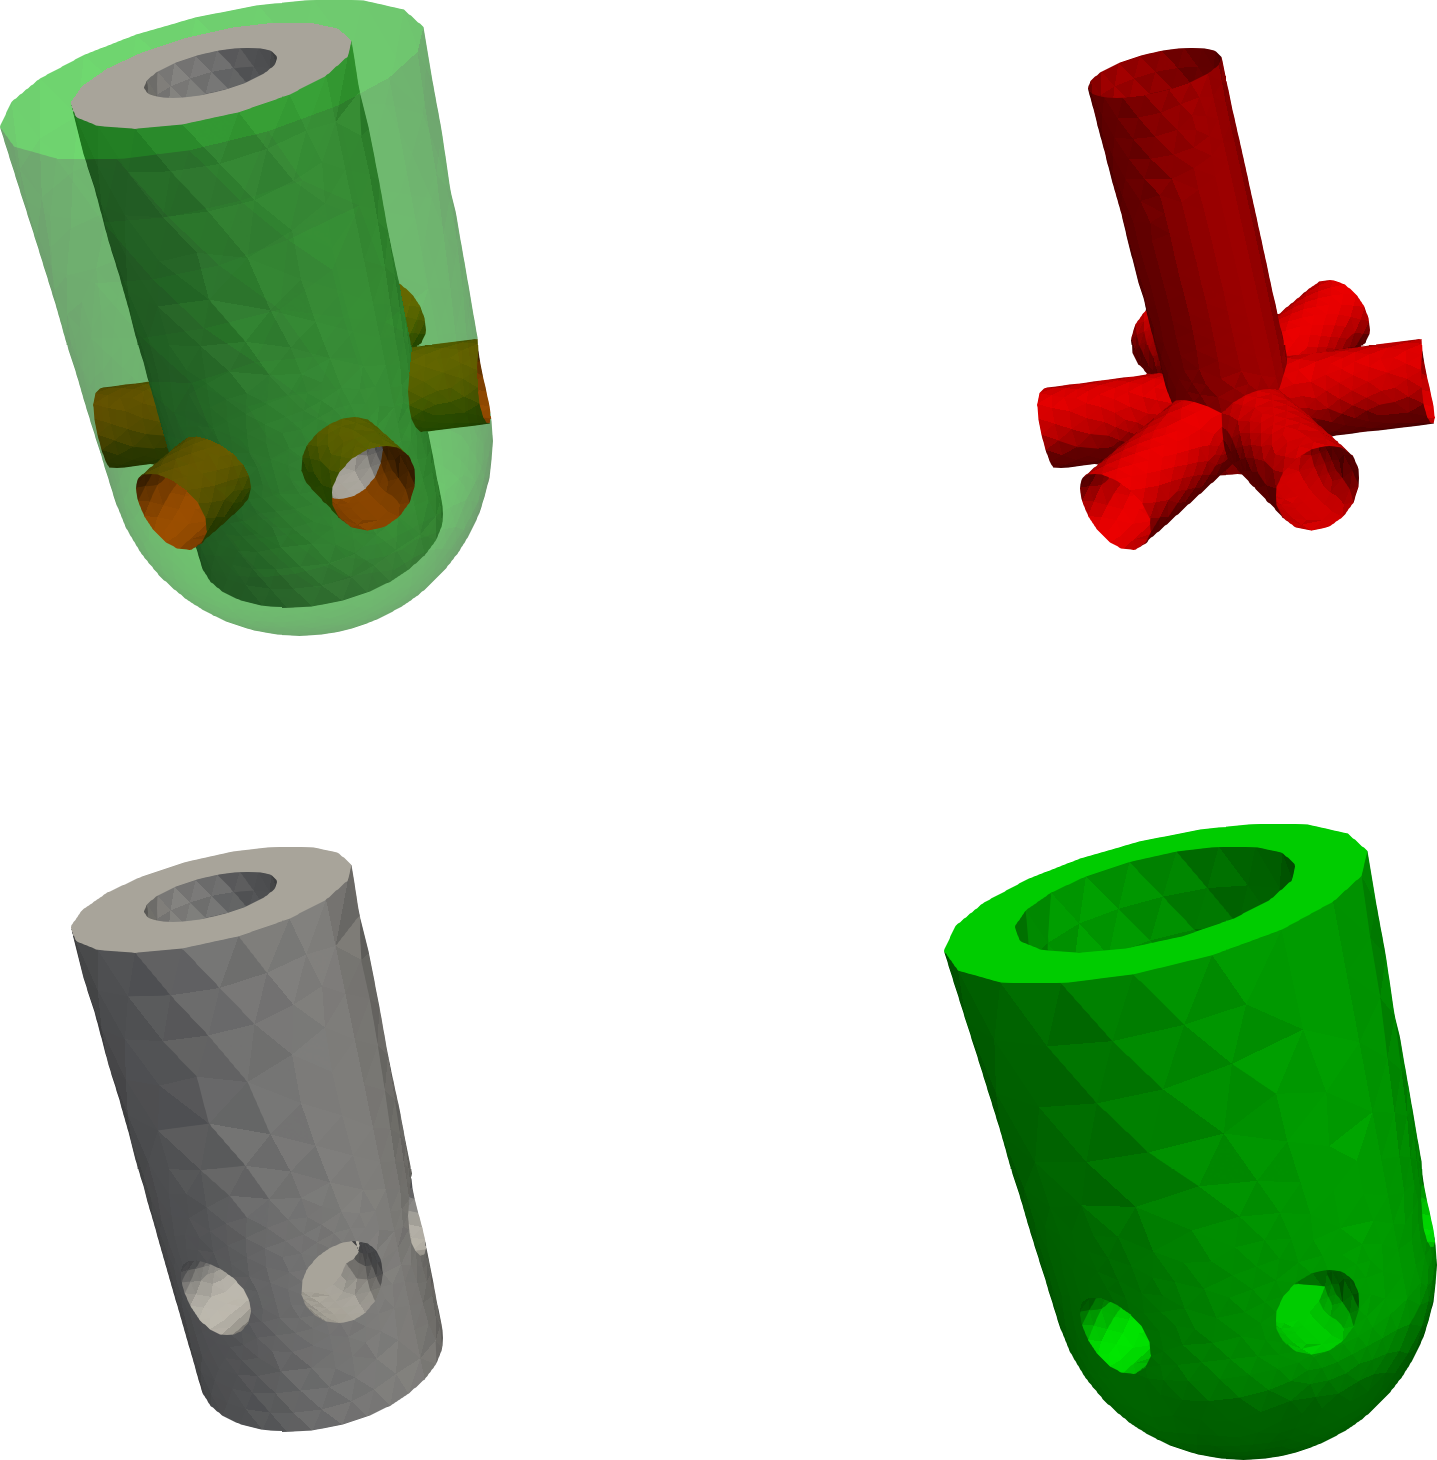
\includegraphics[width=0.5\columnwidth]{img/rfa/catheter}
    \caption{The components of the catheter tip: the inner channels in red, the thermistor in gray and the electrode in green.}
    \label{fig_rfa_catheter}
\end{wrapfloat}

Other works in the literature presented simulations of similar scenarios with a much simplified geometry: most in two spatial dimensions, with the ones in three dimensions having no description of the individual outlets of the inner channels, but instead a contiguous inlet surface going around the whole electrode.
An important improvement in our model, in particular in the geometrical description, was to use meshes of very accurate geometries that resolved all the details of the catheter.
We identify all the main parts of the catheter: the body, the electrode, the thermistor and the channels, with the electrode and the thermistor being part of the actual computational domain while the body and the inner channels are not but shape the boundary of the domain.

\subsection{External factors calibration}
\label{sub_rfaExternalFactors}
As far as the computational domain we used is concerned, it is composed by several additional parts.
The catheter is inserted in a part of the domain occupied by blood, with its tip, the electrode, touching another part, occupied by the tissue.
The tissue part is then resting on an additional part, which we call the \emph{external factors board}, or \emph{board} for short.
In the experiment, the tissue lied on a methacrylate board and the dispersive electrode, necessary for the ablation, was not placed in direct contact with the tissue but rather under this additional board.
The last part of the computational domain, then, corresponds to this additional object separating the tissue from the electrode.
I would like to point out that a similar situation happens in the administration of the real procedure where the dispersive electrode is placed on the patient, usually on the back, again rather far from the heart.

With the addition of this board, the computational domain looks like in Figure~\ref{fig_rfa_compDomain}, where we also reported its physical dimensions in meters for comparison.
\begin{wrapfloat}{figure}{O}{0pt}
  \centering
    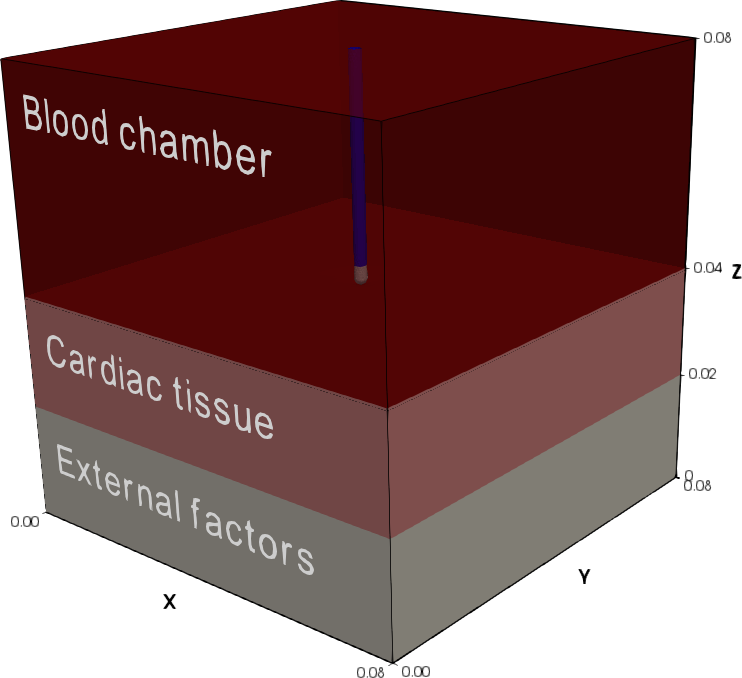
\includegraphics[width=0.5\columnwidth]{img/rfa/compDomain}
    \caption{The computational domain used for our simulations, consisting of the catheter in the blood chamber, with its tip touching the cardiac tissue, which is resting on the external factors board. Dimensions in meters.}
    \label{fig_rfa_compDomain}
\end{wrapfloat}

The presence of the external factors board also gives us the opportunity to calibrate the model to match the setup of the actual experiment, and this is where it gets its name from.
The domain we used in our simulations is much smaller than the actual domain used for the experiments.
This poses a problem as some of the electric power is dissipated outside the small volume we simulate, but it is difficult to keep track of it.
Luckily, we know from the RFA machine how much resistance the whole setup offers to it, so we can tune the \(\sigma\) of the board in order to match the same value.
This gives us a single parameter to tune the computational domain to simulate a much bigger volume; furthermore, the tuning is done only at the beginning of the simulation and then kept throughout the whole run.
I wish to note that the constraint of matching the system's impedance is very important because it ensures that the correct amount of power is distributed to the various components of the domain -- the blood, the tissue, etcetera -- so much so that in a previous work the same goal was achieved by changing the electrical impedance of the cardiac tissue.
Our solution is more elegant and does not affect the physical properties of the parts of the system we are more interested into; we therefore consider it a significant improvement over the state of the art.

\subsection{Elastic contact}
\label{sub_rfaElastic}
The tip of the electrode is in direct contact with the tissue.
During our investigation of the numerical simulation of RFA, it became clear how the geometry of this contact is of the utmost importance for an accurate simulation of the ablation procedure.
The reason is that the part of the electrode surface that is in contact with the tissue will provide electric current directly to it, while the part that is in contact with the blood will dissipate energy into the blood.
Electrons on the electrode, on which they can move freely as it is a good conductor, are in fact faced with the choice of flowing either in the blood or in the tissue.
We know from the theory of electromagnetism that electrons will flow into a medium in an amount directly proportional to the cross-sectional area of the medium and inversely proportional to its impedance; in other words, electrons will favour a medium that they can access through a large area and offers small resistance.
The setting can be modelled as an electric circuit in which current can flow in two parallel branches, one containing a resistance representing the tissue, the other containing a resistance representing the blood and the tissue in a sequence.
As detailed in the paper, we use this description to find that the power dissipated in the tissue is proportional to
\begin{equation}
  \alpha := \frac{A_{tissue}\sigma_{tissue}}{A_{blood}\sigma_{blood} + A_{tissue}\sigma_{tissue}}
  \label{eq_rfaPowerDistribution}
\end{equation}
It is clear that, to correctly reproduce a cardiac ablation, it is essential to know how much of the electrode is in contact with the tissue and how much with the blood; in other words, we need to know the geometry of the electrode-tissue contact, or our simulation, even with all the correct values for the various physical parameters, will behave differently from reality.
It is important to highlight that the electrode-tissue contact surface depends on the applied pressure which is specified in the RFA protocol.

We introduced a model of elastic contact to take this fact into account.
We modelled the configuration as an indentation problem of a rigid sphere -- the catheter tip -- into a half-space -- the cardiac tissue.
We chose to use an elastic material description for the tissue as this gives us the opportunity to use realistic values for the Young modulus and the Poisson ratio that are known in the literature, and also because it is a reasonable choice.
We borrowed knowledge from contact mechanics and described our indentation problem via an \emph{axisymmetric Boussinesq formulation}, which gives us the profile of the tissue surface for a given applied force. 
\begin{figure}
  \centering
    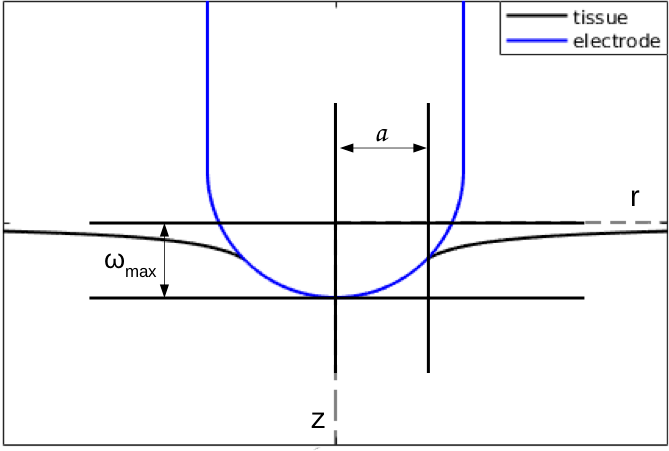
\includegraphics[width=0.75\columnwidth]{img/rfa/crossSectionContact}
    \caption{Sketch of the elastic contact profile: the tissue surface deforms to follow the indenting sphere.}
    \label{fig_rfa_crossSectionContact}
\end{figure}
Prior to the use of contact mechanics to compute a contact profile, numerical models of RFA simply considered a sharp insertion of the catheter into the tissue, meaning that the penetration depth of the catheter into the tissue was adjusted based on the exerted force, but the tissue surface was left unchanged (flat).
This led to an intrinsic overestimation of the electrode-tissue surface contact area that jeopardised the physics of the whole system.
A visual comparison of the two methods will make the difference clear: Figure~\ref{fig_rfa_tissueComparison} presents such comparison.
\begin{figure}
  \centering
    \subfloat[][\SI{10}{g} sharp.\label{fig_rfa_tissueSharp10g}]
    {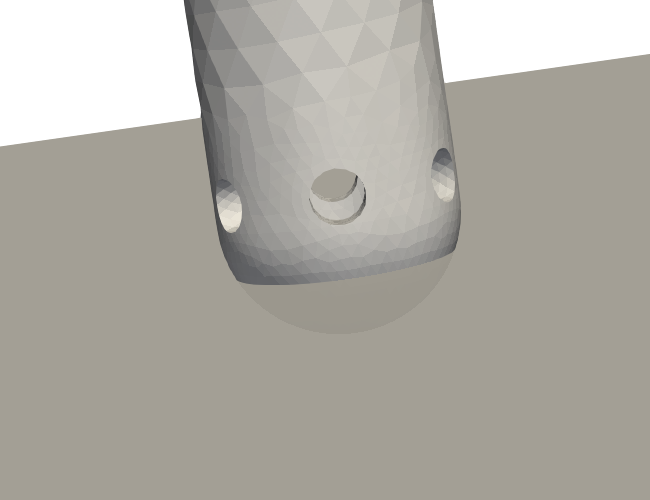
\includegraphics[width=0.3\textwidth]{img/rfa/tissueSharp10g}}
    \quad
    \subfloat[][\SI{20}{g} sharp.\label{fig_rfa_tissueSharp20g}]
    {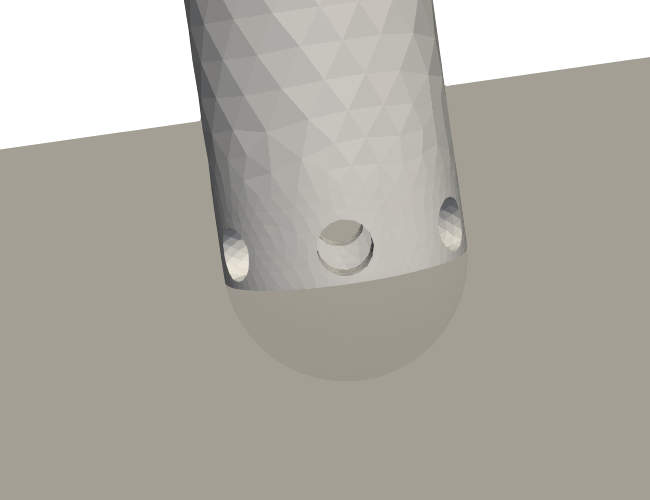
\includegraphics[width=0.3\textwidth]{img/rfa/tissueSharp20g}}
    \quad
    \subfloat[][\SI{40}{g} sharp.\label{fig_rfa_tissueSharp40g}]
    {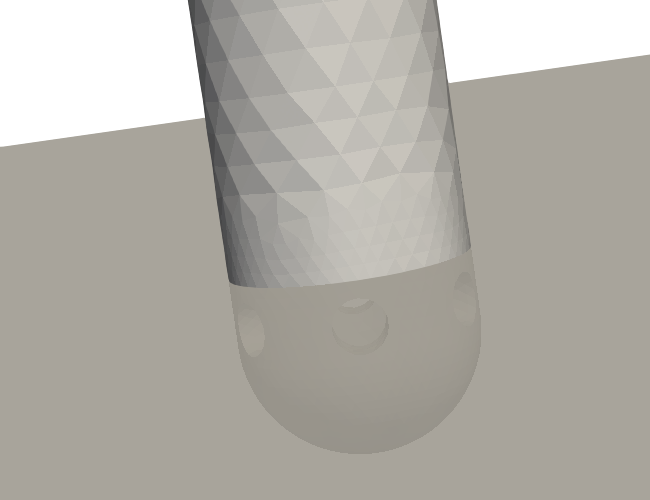
\includegraphics[width=0.3\textwidth]{img/rfa/tissueSharp40g}}
    \\
    \subfloat[][\SI{10}{g} elastic.\label{fig_rfa_tissueElastic10g}]
    {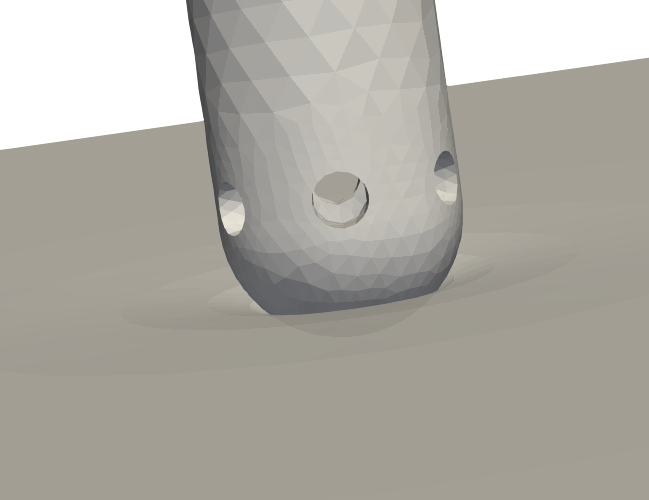
\includegraphics[width=0.3\textwidth]{img/rfa/tissueElastic10g}}
    \quad
    \subfloat[][\SI{20}{g} elastic.\label{fig_rfa_tissueElastic20g}]
    {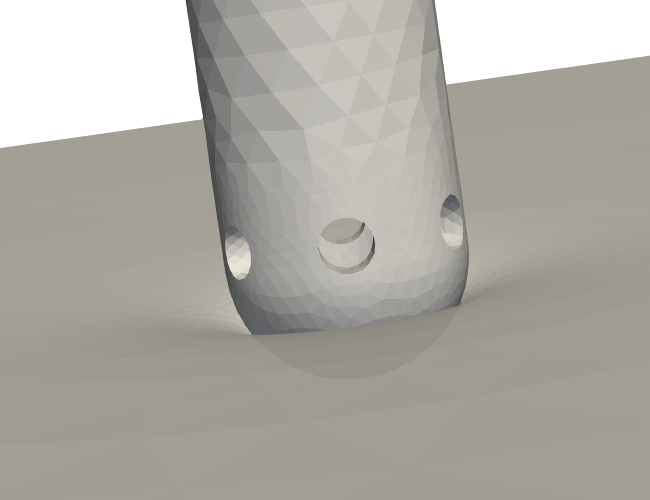
\includegraphics[width=0.3\textwidth]{img/rfa/tissueElastic20g}}
    \quad
    \subfloat[][\SI{40}{g} elastic.\label{fig_rfa_tissueElastic40g}]
    {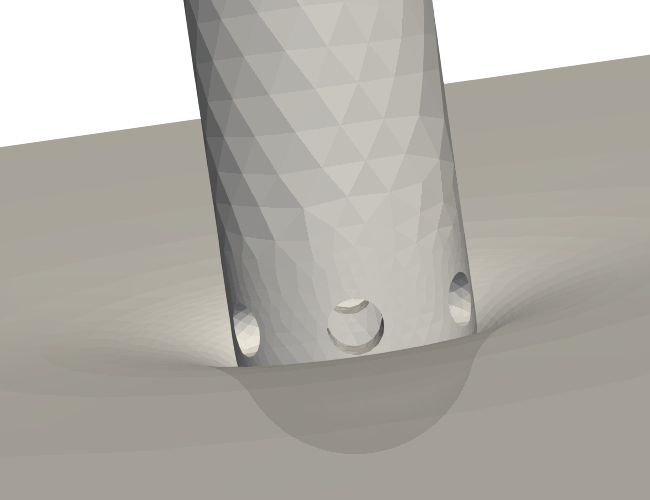
\includegraphics[width=0.3\textwidth]{img/rfa/tissueElastic40g}}
    \caption{Comparison of tissue-catheter contacts for sharp (top row) and elastic (bottom row) contact deformation models for three common values of pressure.}
    \label{fig_rfa_tissueComparison}
\end{figure}
The above discussion should now make sense: it immediately strikes the eye how one of the two approaches, the one represented in the bottom row of pictures, is more realistic.
If the difference is not dramatic in the \SI{10}{g} case, it is in the other two, especially in the \SI{40}{g} case where the displacement is such that the irrigation holes end up under the tissue surface, a clearly unphysical scenario.
The elastic deformation model that we introduced gives a much more realistic approximation of the electrode-tissue contact, resulting in a correct distribution of the electric current between the blood and the tissue.

I want to stress that the misbehavior caused by a computational mesh with an incorrect electrode-tissue contact is not caused by a parameter that can be tuned in the code, because it is a property of the shape of the solution to Equation~\eqref{eq_rfaPotential}.
Although one can still, despite an incorrect geometry, manage to deliver the correct amount of power to the tissue, this will affect the results of the simulation in the rest of the domain, for example in the blood, and ultimately deteriorate the physical accuracy of the simulation in a way that cannot be corrected.

Adding our elastic contact model was a crucial step toward a successful model and was very effective, while it also helped us better understand the physics of the radiofrequency ablation problem.


\subsection{Model summary}
\label{sub_rfaSummary}
Our model is ruled by Equations~\eqref{eq_rfaNS}, \eqref{eq_rfaPotential} and \eqref{eq_rfaBioheat} on a mesh generated according to the discussion in the preceding subsections.
These equations are equipped with a variety of boundary conditions: Figure~\ref{fig_rfa_bcs} shows a schematic representation of the domain, a detail of the catheter tip and all boundary conditions that differ from no-slip (\(\vec{u} = \vec{0}\)), zero current flux (\(\sigma(T)\grad\Phi \cdot \vec{n} = 0\)) and body temperature (\(T = T_b\)).
\begin{figure}
  \centering
    \def\svgwidth{\columnwidth}
    \input{img/rfa/bcs.pdf_tex}
    \caption{Schematic representation of our geometry and boundary conditions that differ from no-slip (\(\vec{u} = \vec{0}\)), zero current flux (\(\sigma(T)\grad\Phi \cdot \vec{n} = 0\)) and body temperature (\(T = T_b\)). On the right, a detail of the catheter's tip in front and top view.}
    \label{fig_rfa_bcs}
\end{figure}
In this figure, \(\vec{u}_{in}\) is the blood's inflow velocity, \(V_0\) is the applied potential, \(\vec{u}_s\) is the saline's inflow velocity and \(T_s\) is its temperature.

The choice of zero current flux on the boundaries of the domain is motivated by the need to make all the current flow to the dispersive electrode, which is what happens in reality.
However, the real domain is much bigger than the computational one from which some current should leave, so an even better approach would be to try and estimate the current that leaves our small domain and impose that flux on the boundary instead.

\section{Experimental setup and data}
\label{sec_experiment}
A good model is not very incisive if it does not match experimental data, which in the case of clinical procedures is often scarce.
In the case of RFA, luckily, we had access to an experimental facility where we performed test ablations in order to collect data.
These tests were not performed on humans, but rather on porcine cardiac tissue; this only affects the values of some physical parameters that we input to the code, but not the general idea and validity of our model.
The experimental setup consists of the catheter and the cardiac tissue, which is resting on a plastic slab.
This setup is submerged into a blood bath, which in turn is contained in a thermal reservoir.
A blood pump circulates the blood to simulate the flow of blood typical of a living patient, which is the main means of thermal dissipation.
The setup is pictured in Figure~\ref{fig_rfa_experiment}.
\begin{figure}
  \centering
    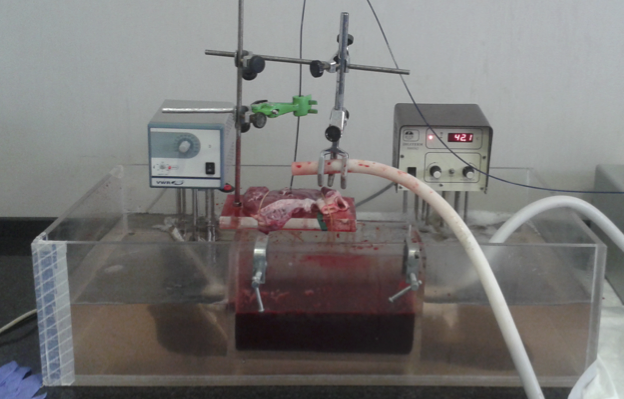
\includegraphics[width=\columnwidth]{img/rfa/experiment}
    \caption{The experimental setup that we aim to reproduce with our model: the tissue and the electrode are submerged in a blood bath where blood flows thanks to a pump.}
    \label{fig_rfa_experiment}
\end{figure}

With this setup, clinicians perform a radiofrequency ablation according to a given protocol on the tissue.
They later cut the tissue open where the ablation was performed and wash it with a special solution that reacts with burnt tissue, making it white.
This makes it possible to have a visual feedback of the lesion that the procedure caused.
Figure~\ref{fig_rfa_lesionExp} shows one such lesion, from the very same set of experiments.
For comparison, Figure~\ref{fig_rfa_lesionSim} shows a similar lesion as a result of a simulation using the model we developed.
\begin{figure}
  \centering
    \subfloat[][Experimental lesion.\label{fig_rfa_lesionExp}]
    {\includegraphics[width=0.45\textwidth]{img/rfa/lesionExp}}
    \quad
    \subfloat[][Simulated lesion.\label{fig_rfa_lesionSim}]
    {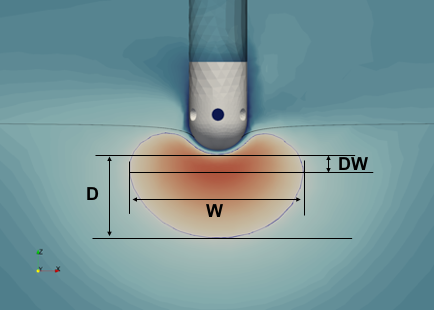
\includegraphics[width=0.45\textwidth]{img/rfa/lesionSim}}
    \caption{A lesion caused to real tissue in an experiment and a simulated lesion obtained with our code. On both figures we defined the quantities of interest that we used to validate our model against the available experimental data.}
    \label{fig_rfa_lesions}
\end{figure}
In Figure~\ref{fig_rfa_lesions} we highlighted the definitions of some quantities of interest that describe a lesion's shape, namely its width (W), its depth (D) and the depth of its maximum width (DW).
These quantities are very meaningful as they can be used to plan an administration of the procedure, and they are easy to compute both in vitro and in silico.
We validated our code and model against this data; all the details are in the attached paper but a brief overview of the results is in Section~\ref{sec_rfaResults}.

\section{Results overview}
\label{sec_rfaResults}
This section contains sample results from simulations of the model introduced in Section~\ref{sec_rfaModel}.
I do not want to delve into the details of data validation in favor of a more qualitative presentation: a quantitative discussion is deferred to the attached paper; here, it is enough to anticipate that we were able to validate the experimental data to a satisfactory level of accuracy.

Instead, I would like to show a typical visualisation of a simulation result.
Figure~\ref{fig_rfa_sim} shows two lesions simulated with protocols that differ in the applied pressure.
\begin{figure}
  \centering
    \subfloat[][\SI{10}{g}\label{fig_rfa_sim10g}]
    {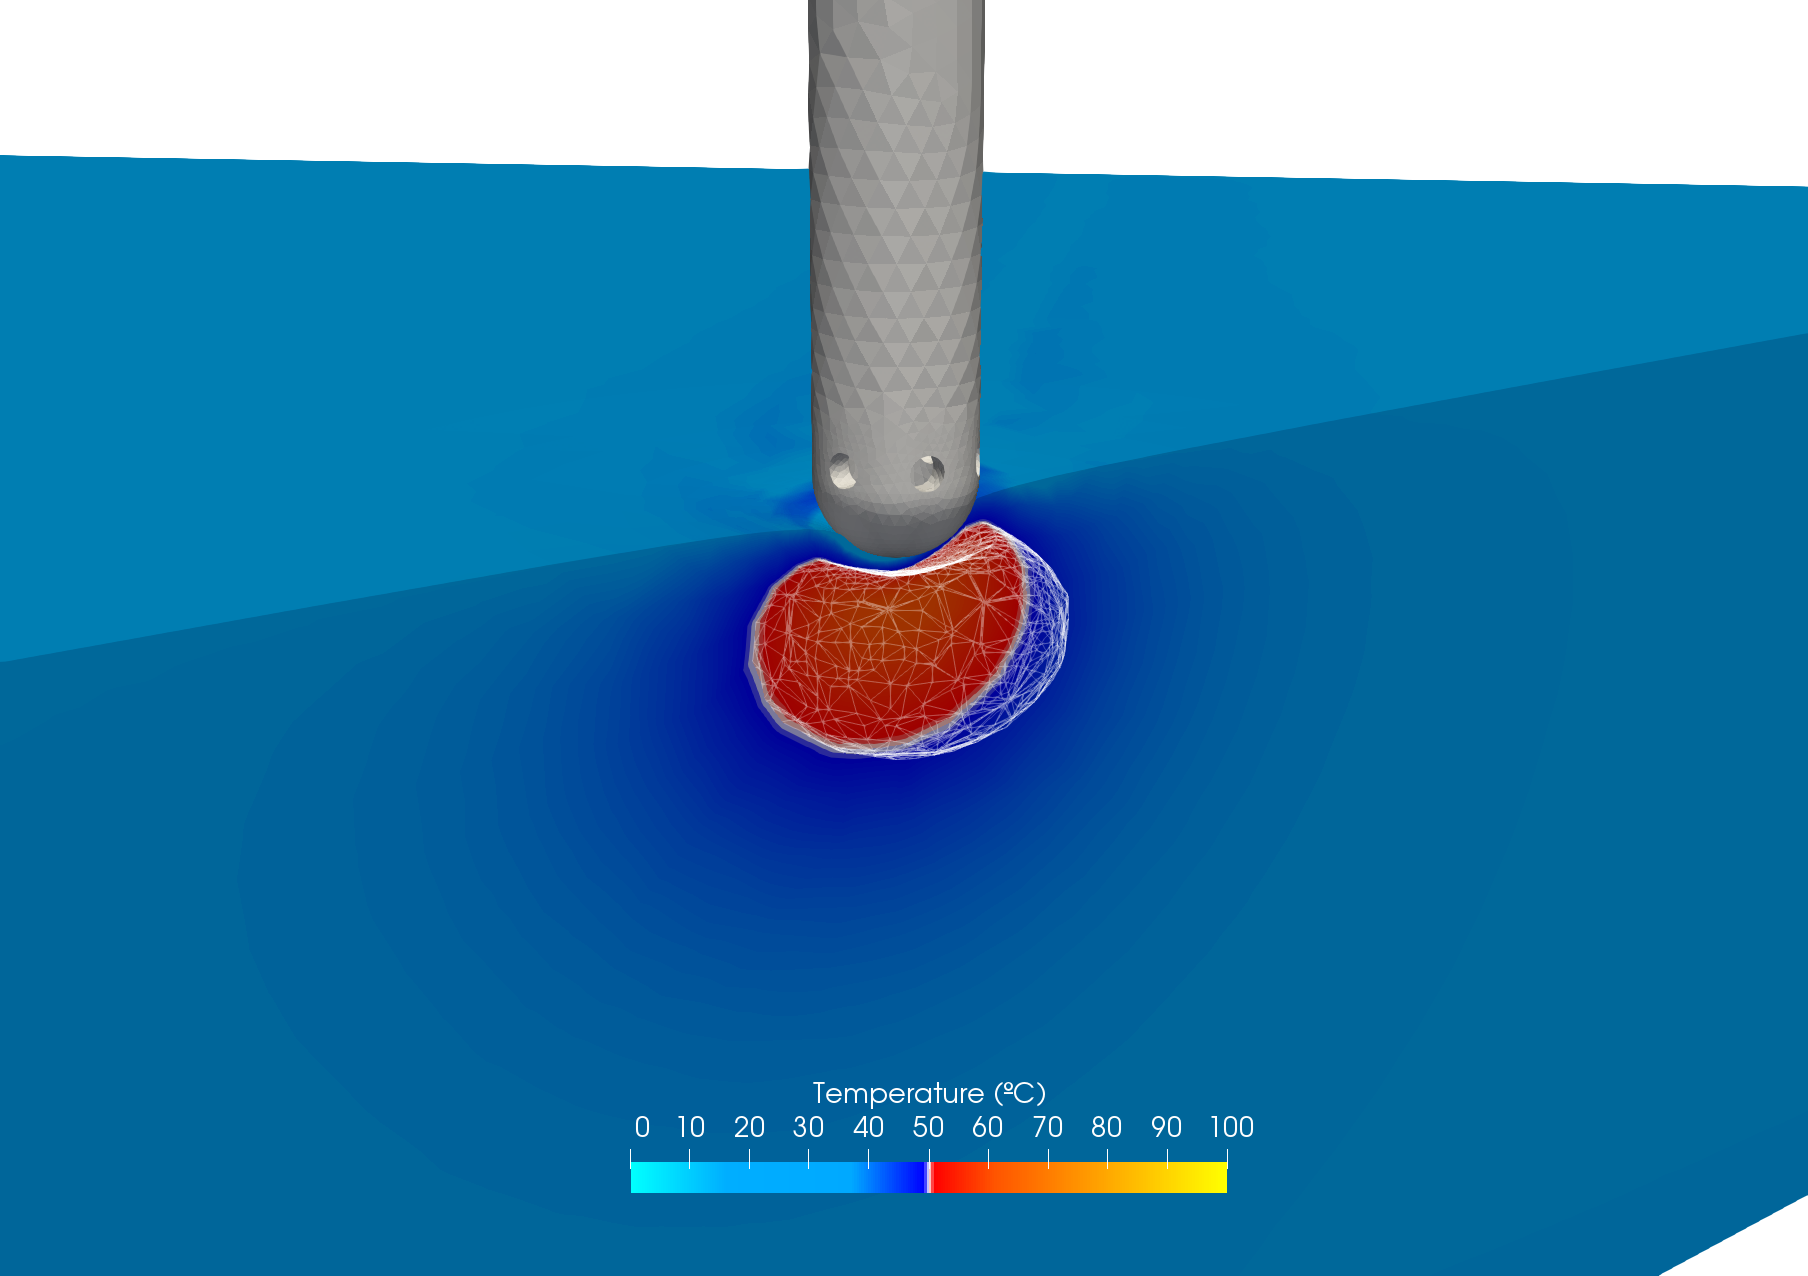
\includegraphics[width=0.45\textwidth]{img/rfa/elastic10g}}
    \quad
    \subfloat[][\SI{40}{g}\label{fig_rfa_sim40g}]
    {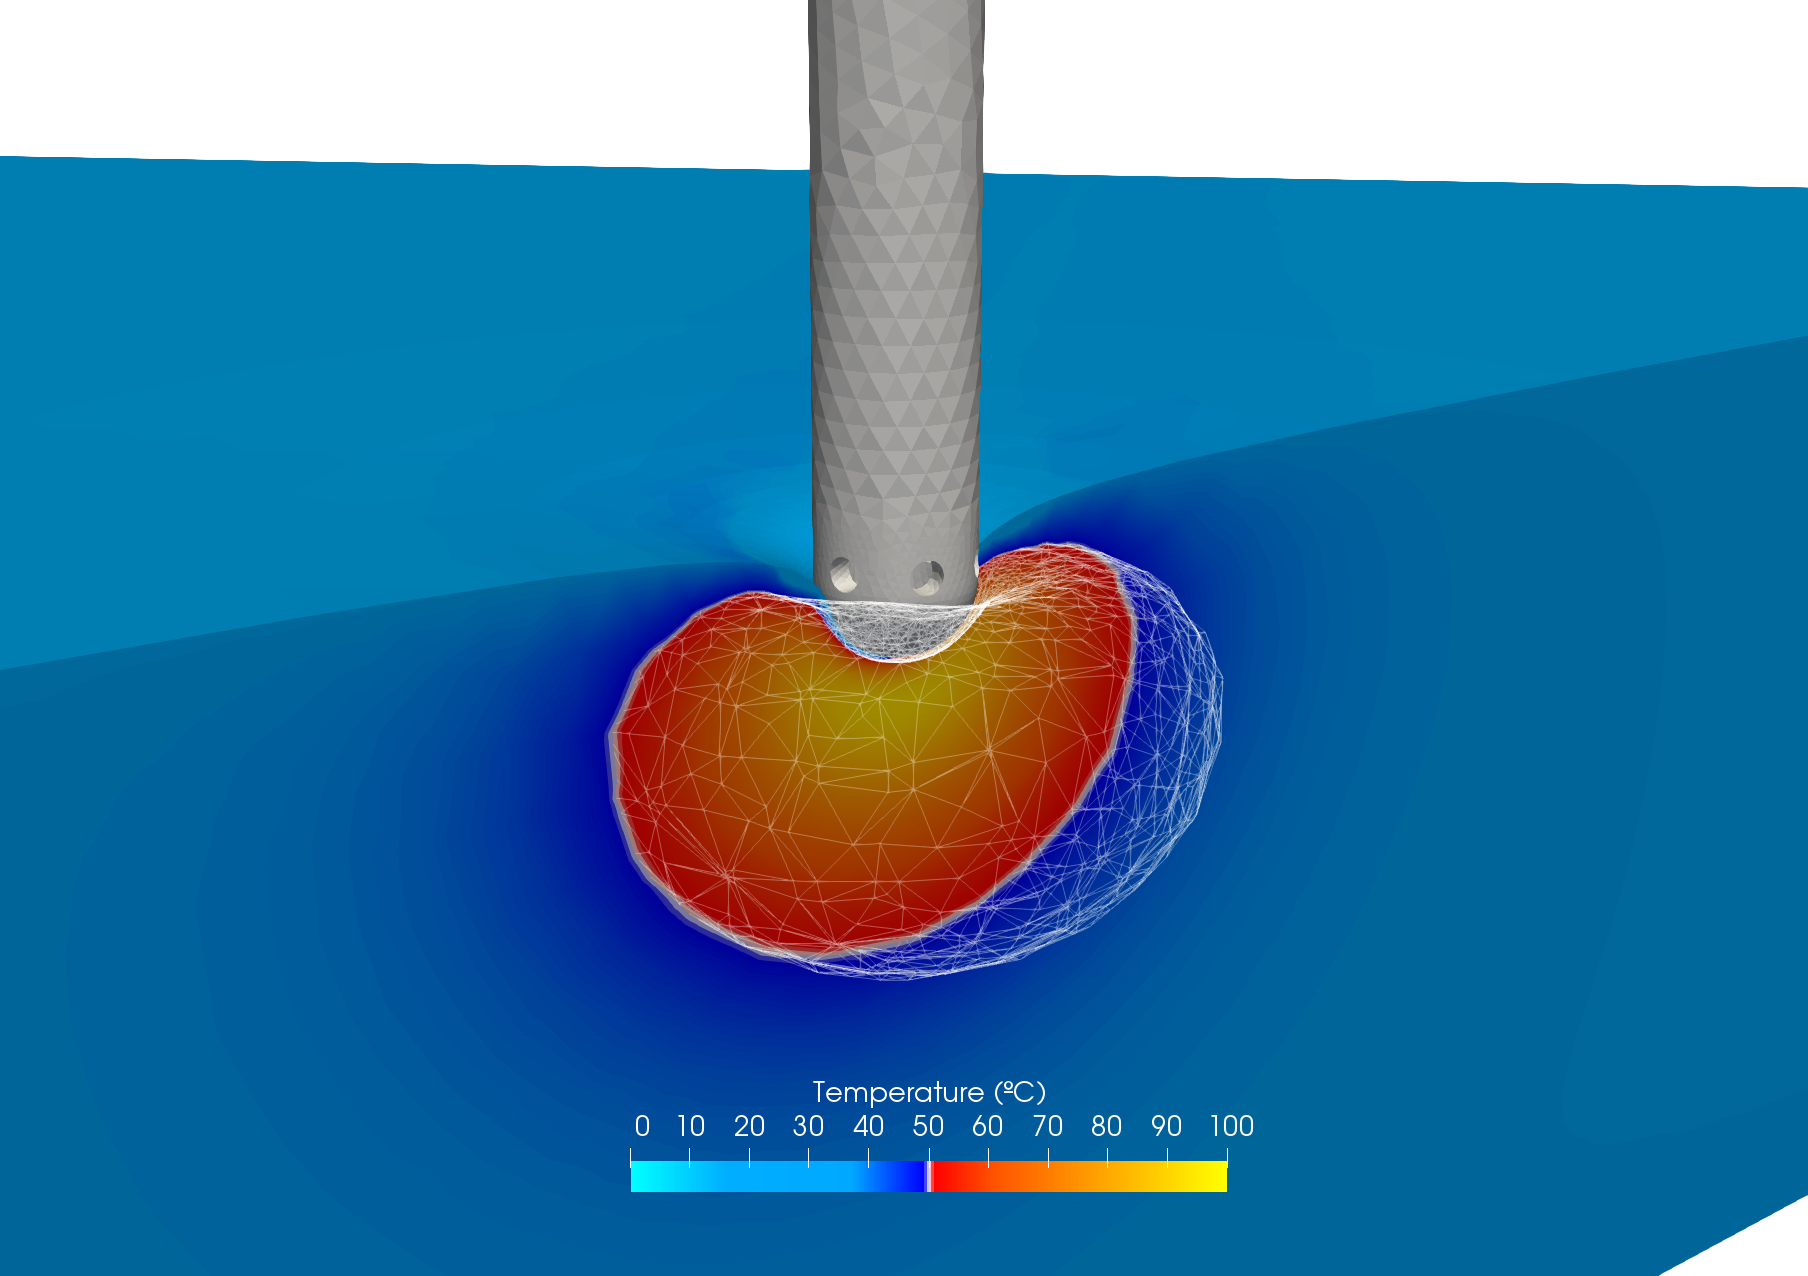
\includegraphics[width=0.45\textwidth]{img/rfa/elastic40g}}
    \caption{Simulated lesions for two protocols at \SI{10}{g} (left) and \SI{40}{g} (right). The view shows a cut through the cardiac tissue and an isosurface at \SI{50}{\celsius} that represents the lesion.}
    \label{fig_rfa_sim}
\end{figure}
The lesions are identified by the white isosurface, while the simulation also gives an estimate of the temperature reached inside the lesion, which is critical as we discussed in Section~\ref{sec_rfa}.
The results are consistent with our expectations: the lesion in Figure~\ref{fig_rfa_sim40g} is much bigger than that in Figure~\ref{fig_rfa_sim10g}, a consequence of the fact that the electrode-tissue contact area is bigger.
Datasets like those behind Figure~\ref{fig_rfa_sim} contain much more information than the various indexes used to estimate the lesion size that I mentioned in Section~\ref{sec_rfaLesion}, making them much more useful for clinical decision-making.
With detailed information on the size of the lesion it is possible to optimally plan the administration of the procedure to reduce the risk for the patient and improve the result.

\section[Future developments]{Cylindrical catheters, high and low flows, high-power ablation and beyond}
\label{sec_future}
Availability of experimental data is often low in medical applications, making it harder to test new protocols or techniques.
A reliable model makes the task easier as it allows to experiment at will in the digital twin with confidence that the behaviour is representative of the actual phenomenon.
For this reason, the model we built can be, and has been, used to test the effects of variations in the geometry, in the parameters, in the protocol, etcetera.
In this section I would like to point out possible present and future research directions that we can follow using the technology we developed.
\begin{itemize}
  \item \textbf{Cylindrical catheters.} The catheters we simulated when testing the model all have a spherical tip, in order to match the one used in the experiments we tried to reproduce. However, cylindrical tips are also common and one might ask if one of is better than the other. Cylindrical tips are flat and their electrode-tissue contact area changes much less with a perturbation in the applied pressure than the one of spherical catheters. Knowing how important the electrode-tissue surface area is, one might argue that cylindrical tips offer more stability in the results being less sensitive to variations in the applied pressure, that are systemic and difficult to eliminate completely. Since simulating a cylindrical tip is very easy with out model, as we only need to provide the code with a corresponding mesh, we can easily investigate this question.
  \item \textbf{High flow and low flow.} The blood flow in the heart during the ablation is the main means of thermal diffusion that, alongside the coolant injected by the catheter, helps to control the temperature rise. In our simulation we mainly used a fixed value for the inlet of the blood flow, a reasonable value that matched the experimental setup. In the human heart, however, the blood velocity varies noticeably from atria to ventricles, and in sedated patients it is likely smaller than in a regular heart. Figure~\ref{fig_rfa_saline} shows how the convection of the saline coolant is affected by the blood flow we routinely used (that we call \emph{high flow}, Figure~\ref{fig_rfa_salineHighFlow}) and by a weaker one (which we refer to as \emph{low flow}, Figure~\ref{fig_rfa_salineLowFlow}).
    \begin{figure}
      \centering
      \subfloat[][High flow\label{fig_rfa_salineHighFlow}]
      {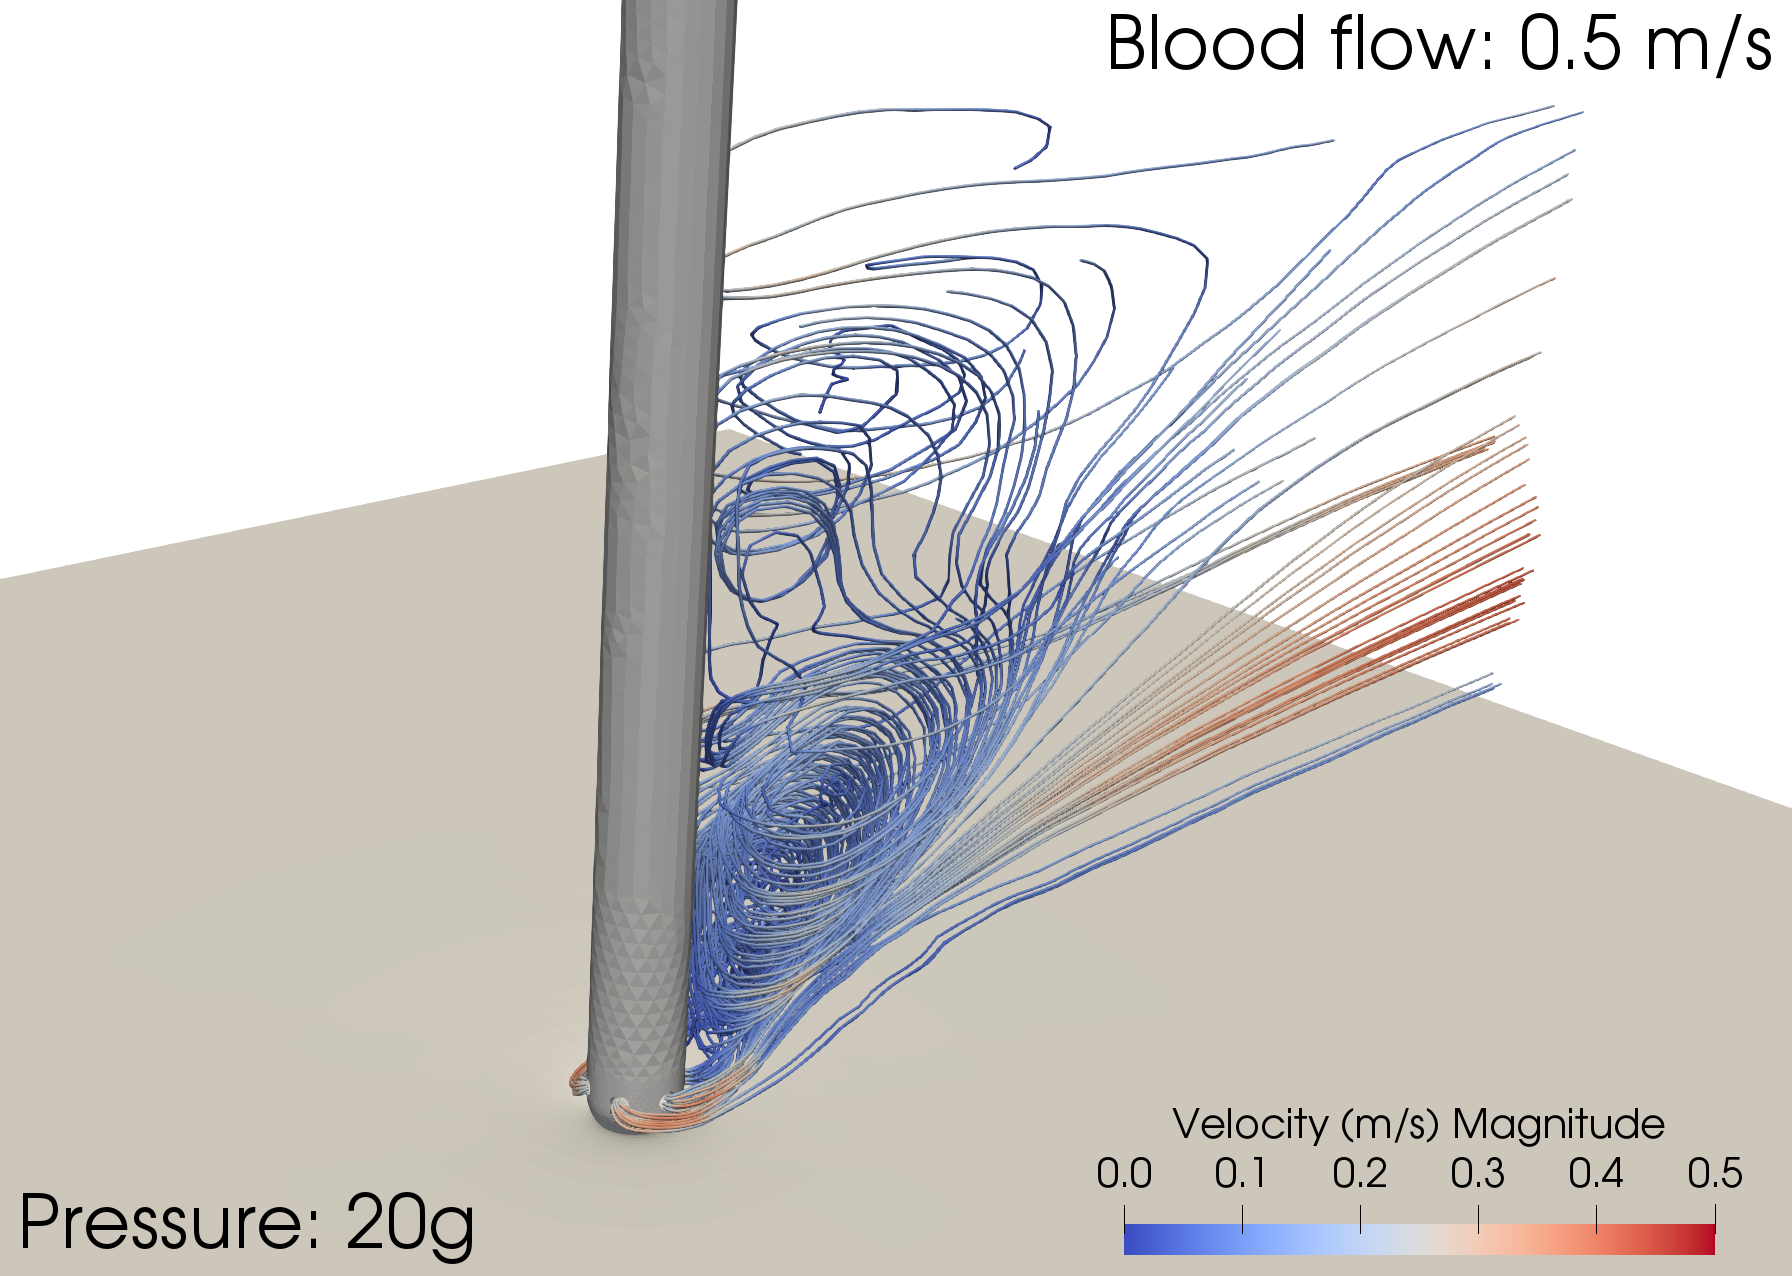
\includegraphics[width=0.45\textwidth]{img/rfa/salineHighFlow}}
      \quad
      \subfloat[][Low flow\label{fig_rfa_salineLowFlow}]
      {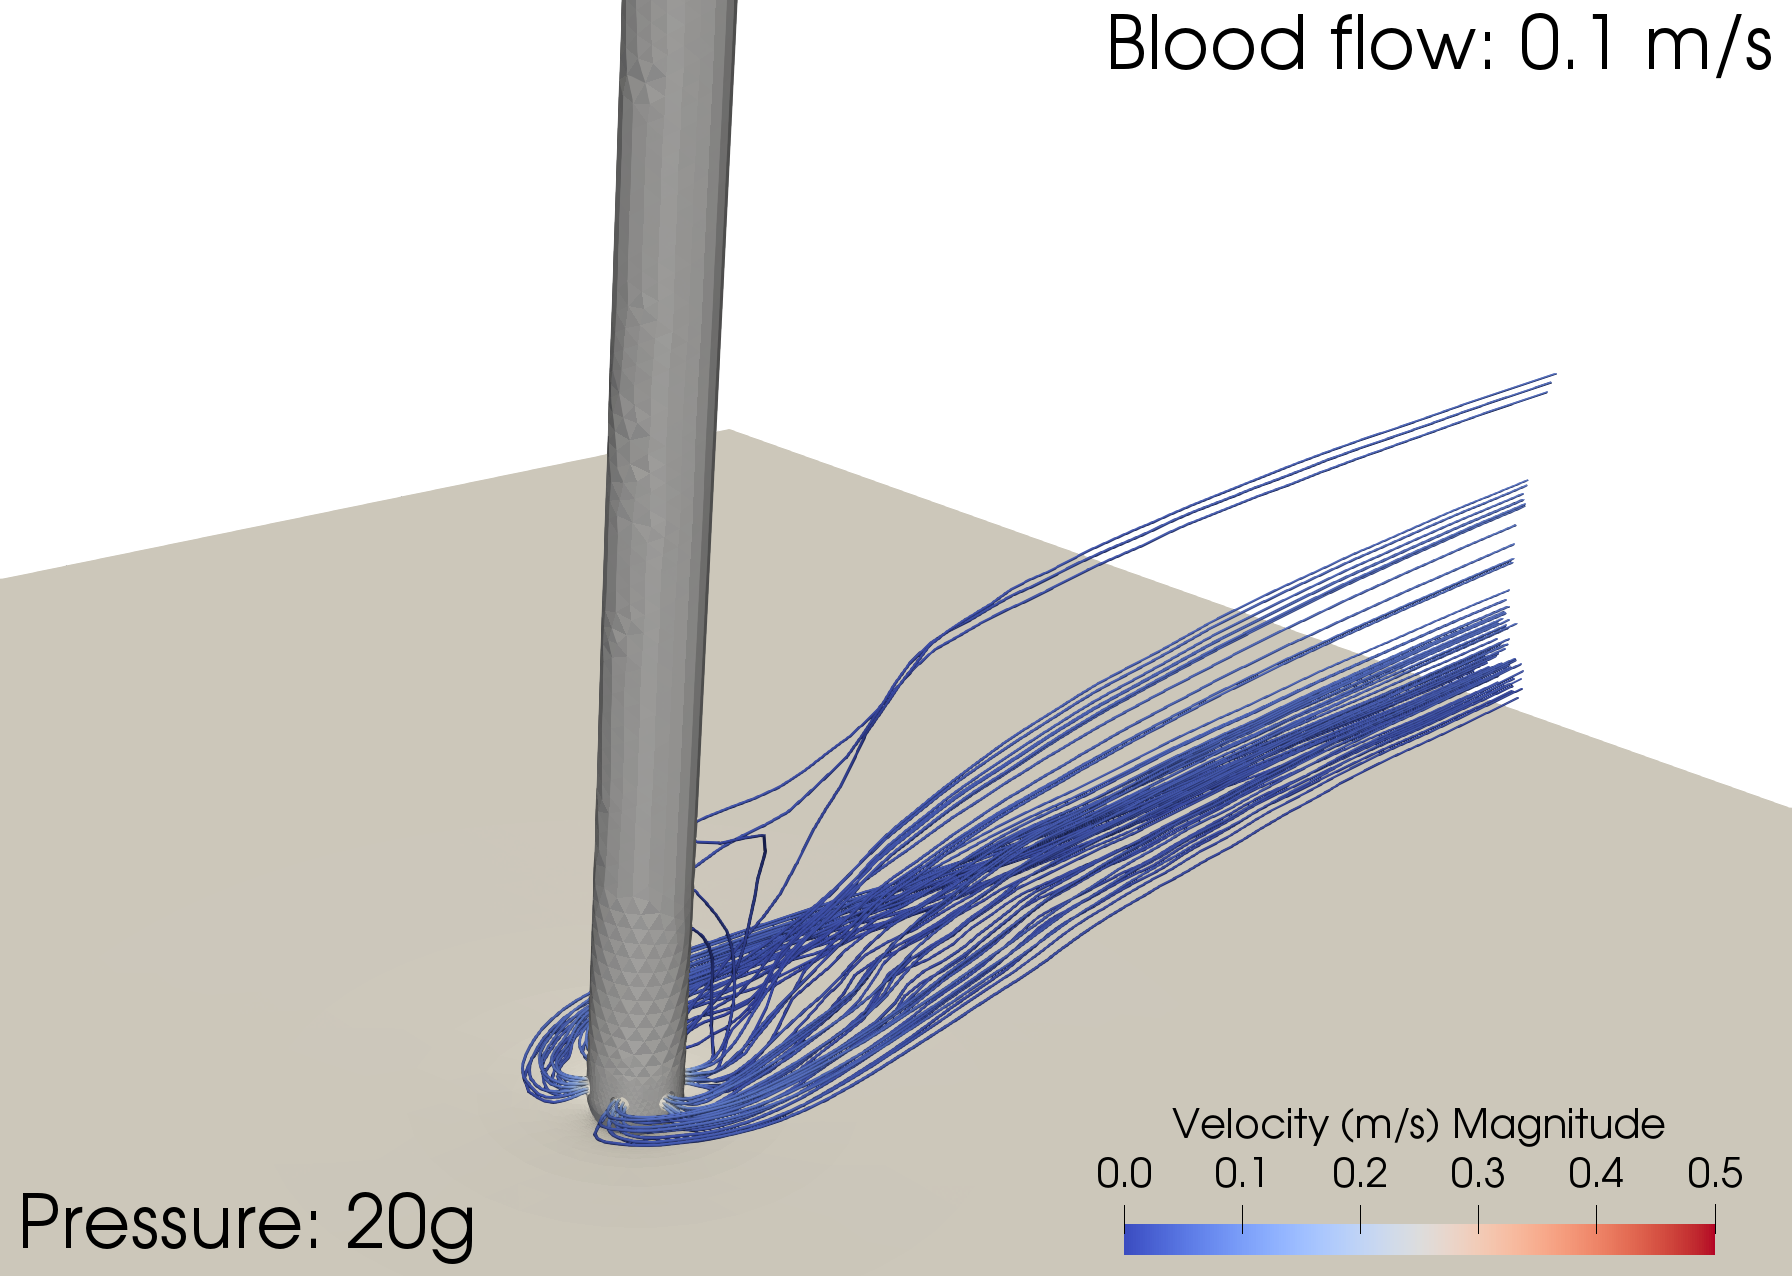
\includegraphics[width=0.45\textwidth]{img/rfa/salineLowFlow}}
      \caption{Convection of the saline coolant with a high flow (left) and a low flow (right) profiles.}
      \label{fig_rfa_saline}
    \end{figure}
    In Figure~\ref{fig_rfa_flowLesions} we show a comparison of lesions from simulations with high and low profiles, in front and lateral views.
    \begin{figure}
      \centering
      \subfloat[][High flow, front view.\label{fig_rfa_flowLesionsHX}]
      {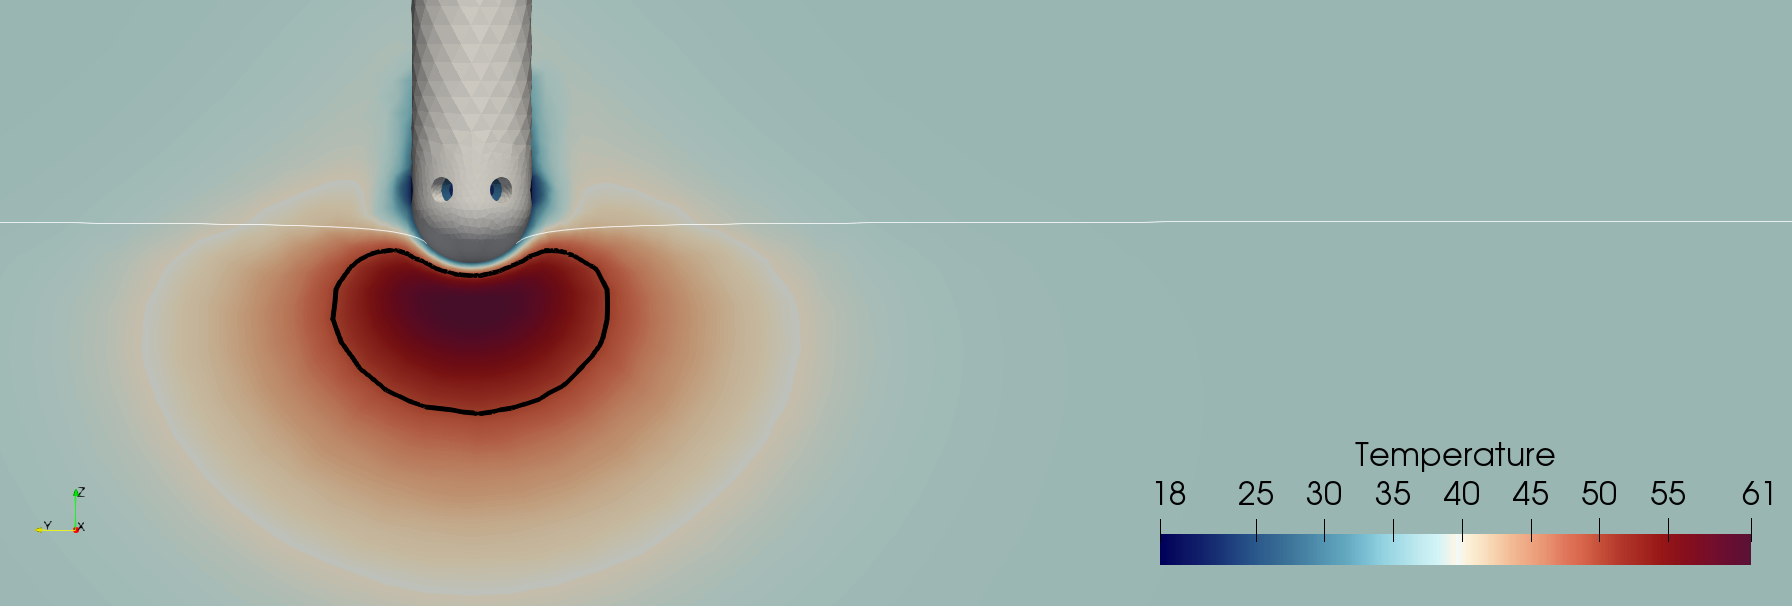
\includegraphics[width=0.45\textwidth]{img/rfa/HF_xaxis}}
      \quad
      \subfloat[][High flow, lateral view.\label{fig_rfa_flowLesionsHY}]
      {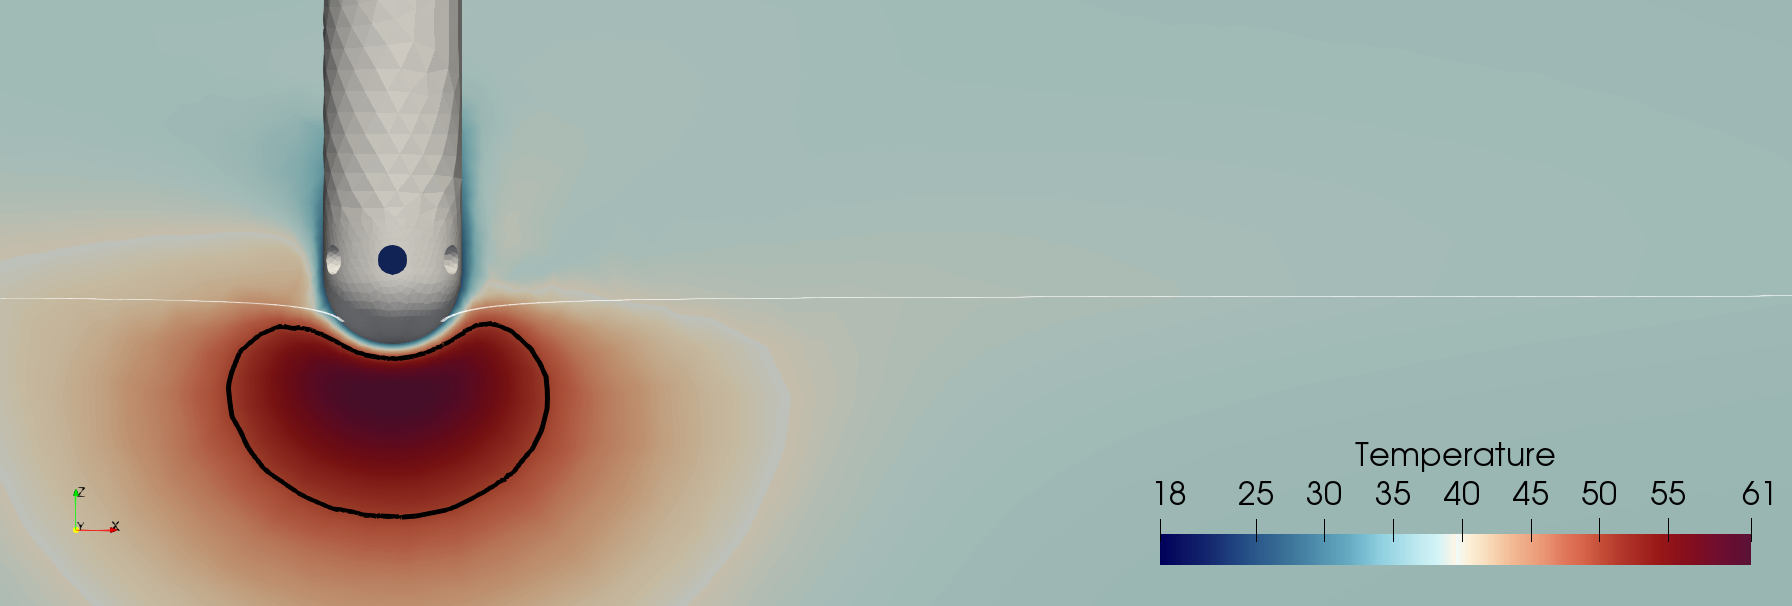
\includegraphics[width=0.45\textwidth]{img/rfa/HF_yaxis}}
      \\
      \subfloat[][Low flow, front view.\label{fig_rfa_flowLesionsLX}]
      {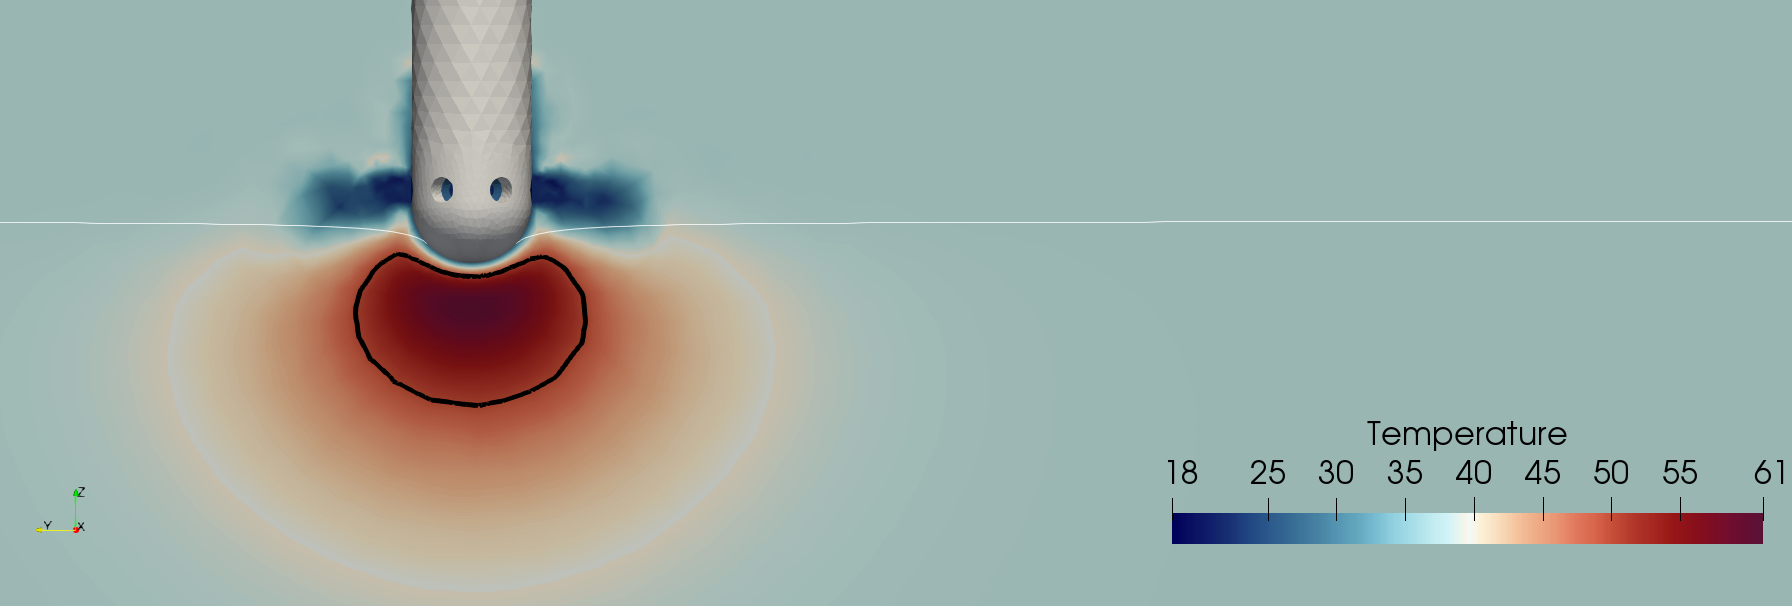
\includegraphics[width=0.45\textwidth]{img/rfa/LF_xaxis}}
      \quad
      \subfloat[][Low flow, lateral view.\label{fig_rfa_flowLesionsLY}]
      {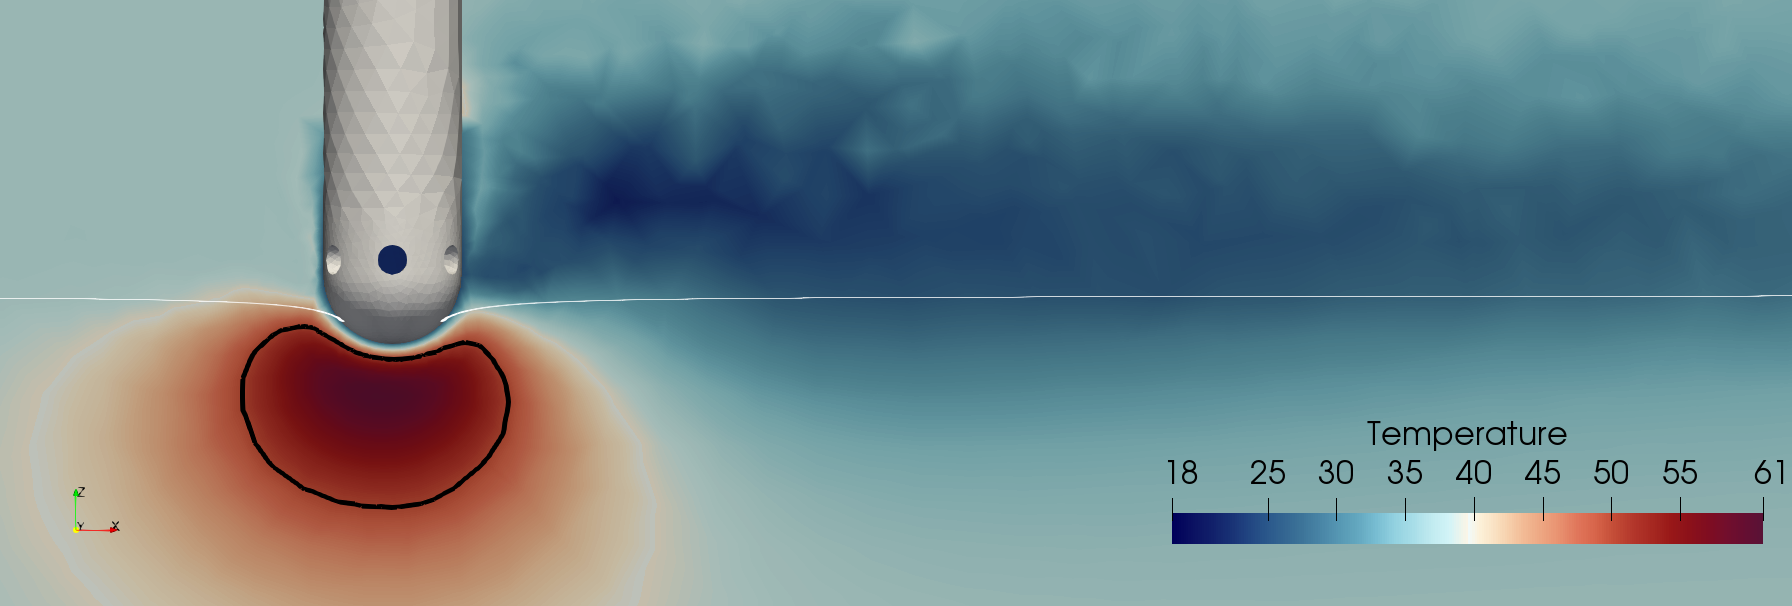
\includegraphics[width=0.45\textwidth]{img/rfa/LF_yaxis}}
      \caption{Lesion comparison with high and low flow profiles.}
      \label{fig_rfa_flowLesions}
    \end{figure}
    Interestingly, a low blood flow makes the coolant more effective as the lesion is overall smaller (Figure~\ref{fig_rfa_flowLesionsHX} versus Figure~\ref{fig_rfa_flowLesionsLX}) and asymmetric, as the cooling becomes more effective in the wake of the cylinder where the coolant stagnates a little longer (Figure~\ref{fig_rfa_flowLesionsHY} versus Figure~\ref{fig_rfa_flowLesionsLY}).
  \item \textbf{High-power ablation.} Recently, clinicians showed a lot of interest for \emph{high-power} ablation protocols, meaning protocols that prescribe ablations dissipating powers in the range \SI{70}{W}-\SI{90}{W}, significantly higher than what is common at the time of writing, but for shorter periods of time. The benefits would include reduced discomfort for the patient, from a shorter procedure, and in general a shorter time window in which complications can arise. We have been experimenting with high-power ablation protocols using our model, collecting results that we will present in an upcoming publication. Again, this only meant changing a number in our configuration and running several simulations.
  \item \textbf{Human versus animal tissue.} The experiments we reproduced were performed on porcine cardiac tissue. However, human cardiac tissue has different mechanical properties and, a priori, it is not clear if the results will be the same in terms of lesion sizes and maximum temperatures. Our model lets us verify this assumption very easily by simply setting different material properties for the tissue, resulting in a different electrode-tissue contact deformation, a parameter to which the simulation results are very sensitive, as we discussed. We collected results on this issue in a scientific contribution that is attached in the second part of this thesis.
\end{itemize}

The list above is not exhaustive and hopes to express the relevance of the model that we implemented and the number of research directions it allows us to investigate.

